Nhóm trình bày sơ lược về quá trình triển khai hệ thống của mình lên heroku. Trước tiên nhóm tạo hai app trên Heroku, một cho front-end ứng với ReactJS và một cho back-end ứng với JavaSpring và PostgreSQL. 

\subsubsection{Front-end}
\begin{enumerate}
    \item Trước tiên, cần tải source code lên Github, sau đó liên kết repo git này với app heroku.
    \item Thêm buildpack react vào app heroku, theo đường dẫn sau: \href{https://github.com/mars/create-react-app-buildpack}{Heroku Buildpack for create-react-app}
    \item Chọn nhánh ở repo Github để tiến hành build.
    \item Cuối cùng là nhấn nút Deploy để tiến hành build lần đầu, sau đó chọn vào ô "Automatic deploys" để app có thể tự động build khi có code mới ở Github. \ref{deploy_front_end}
\end{enumerate}

\begin{figure}[H]
    \begin{center}
        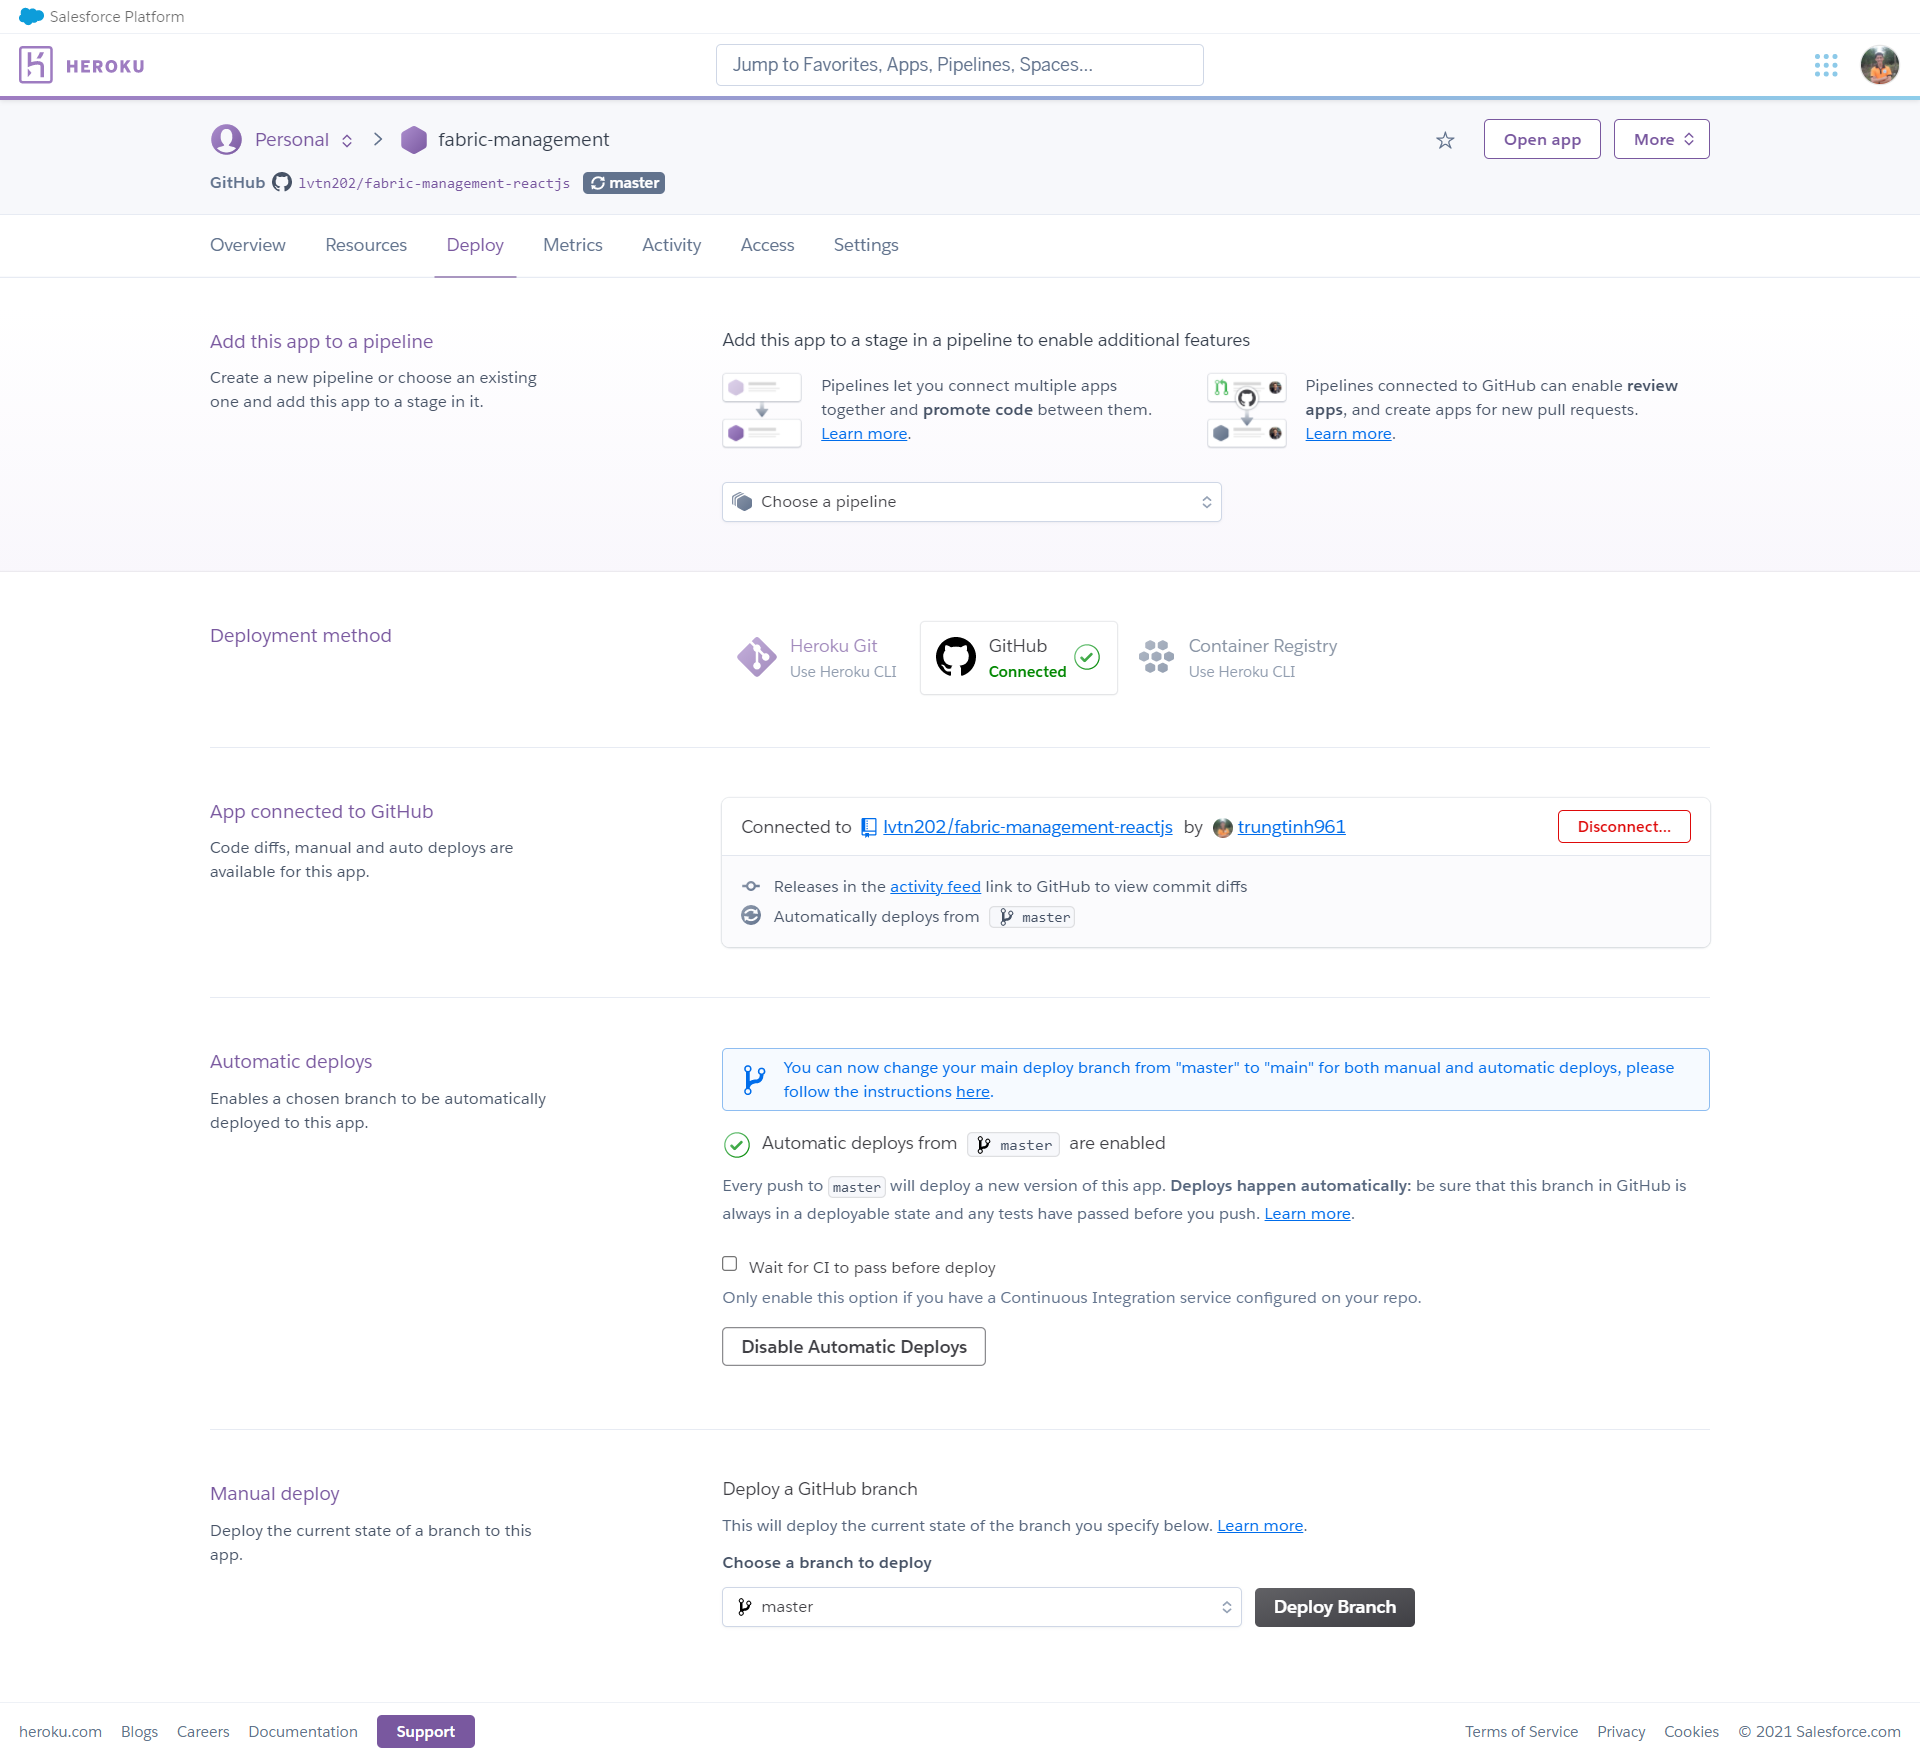
\includegraphics[width=16cm]{Image/Technical/deploy-front-end.png}
        \caption{Deploy Front-end Heroku}
        \label{deploy_front_end}
    \end{center}
\end{figure}

\subsubsection{Back-end}
\begin{enumerate}
    \item Trước tiên, cần tải source code lên Github, sau đó liên kết repo git này với app heroku.
    \item Thêm add-ons Heroku-Postgres vào để lưu trữ CSDL của hệ thống.
    \item Điều chỉnh các thông tin về CSDL trong source code để kết nối đến CSDL trên add-ons vừa thêm.
    \item Chọn nhánh ở repo Github để tiến hành build.
    \item Cuối cùng là nhấn nút Deploy để tiến hành build lần đầu, sau đó chọn vào ô "Automatic deploys" để app có thể tự động build khi có code mới ở Github. \ref{deploy_back_end}
\end{enumerate}

\begin{figure}[H]
    \begin{center}
        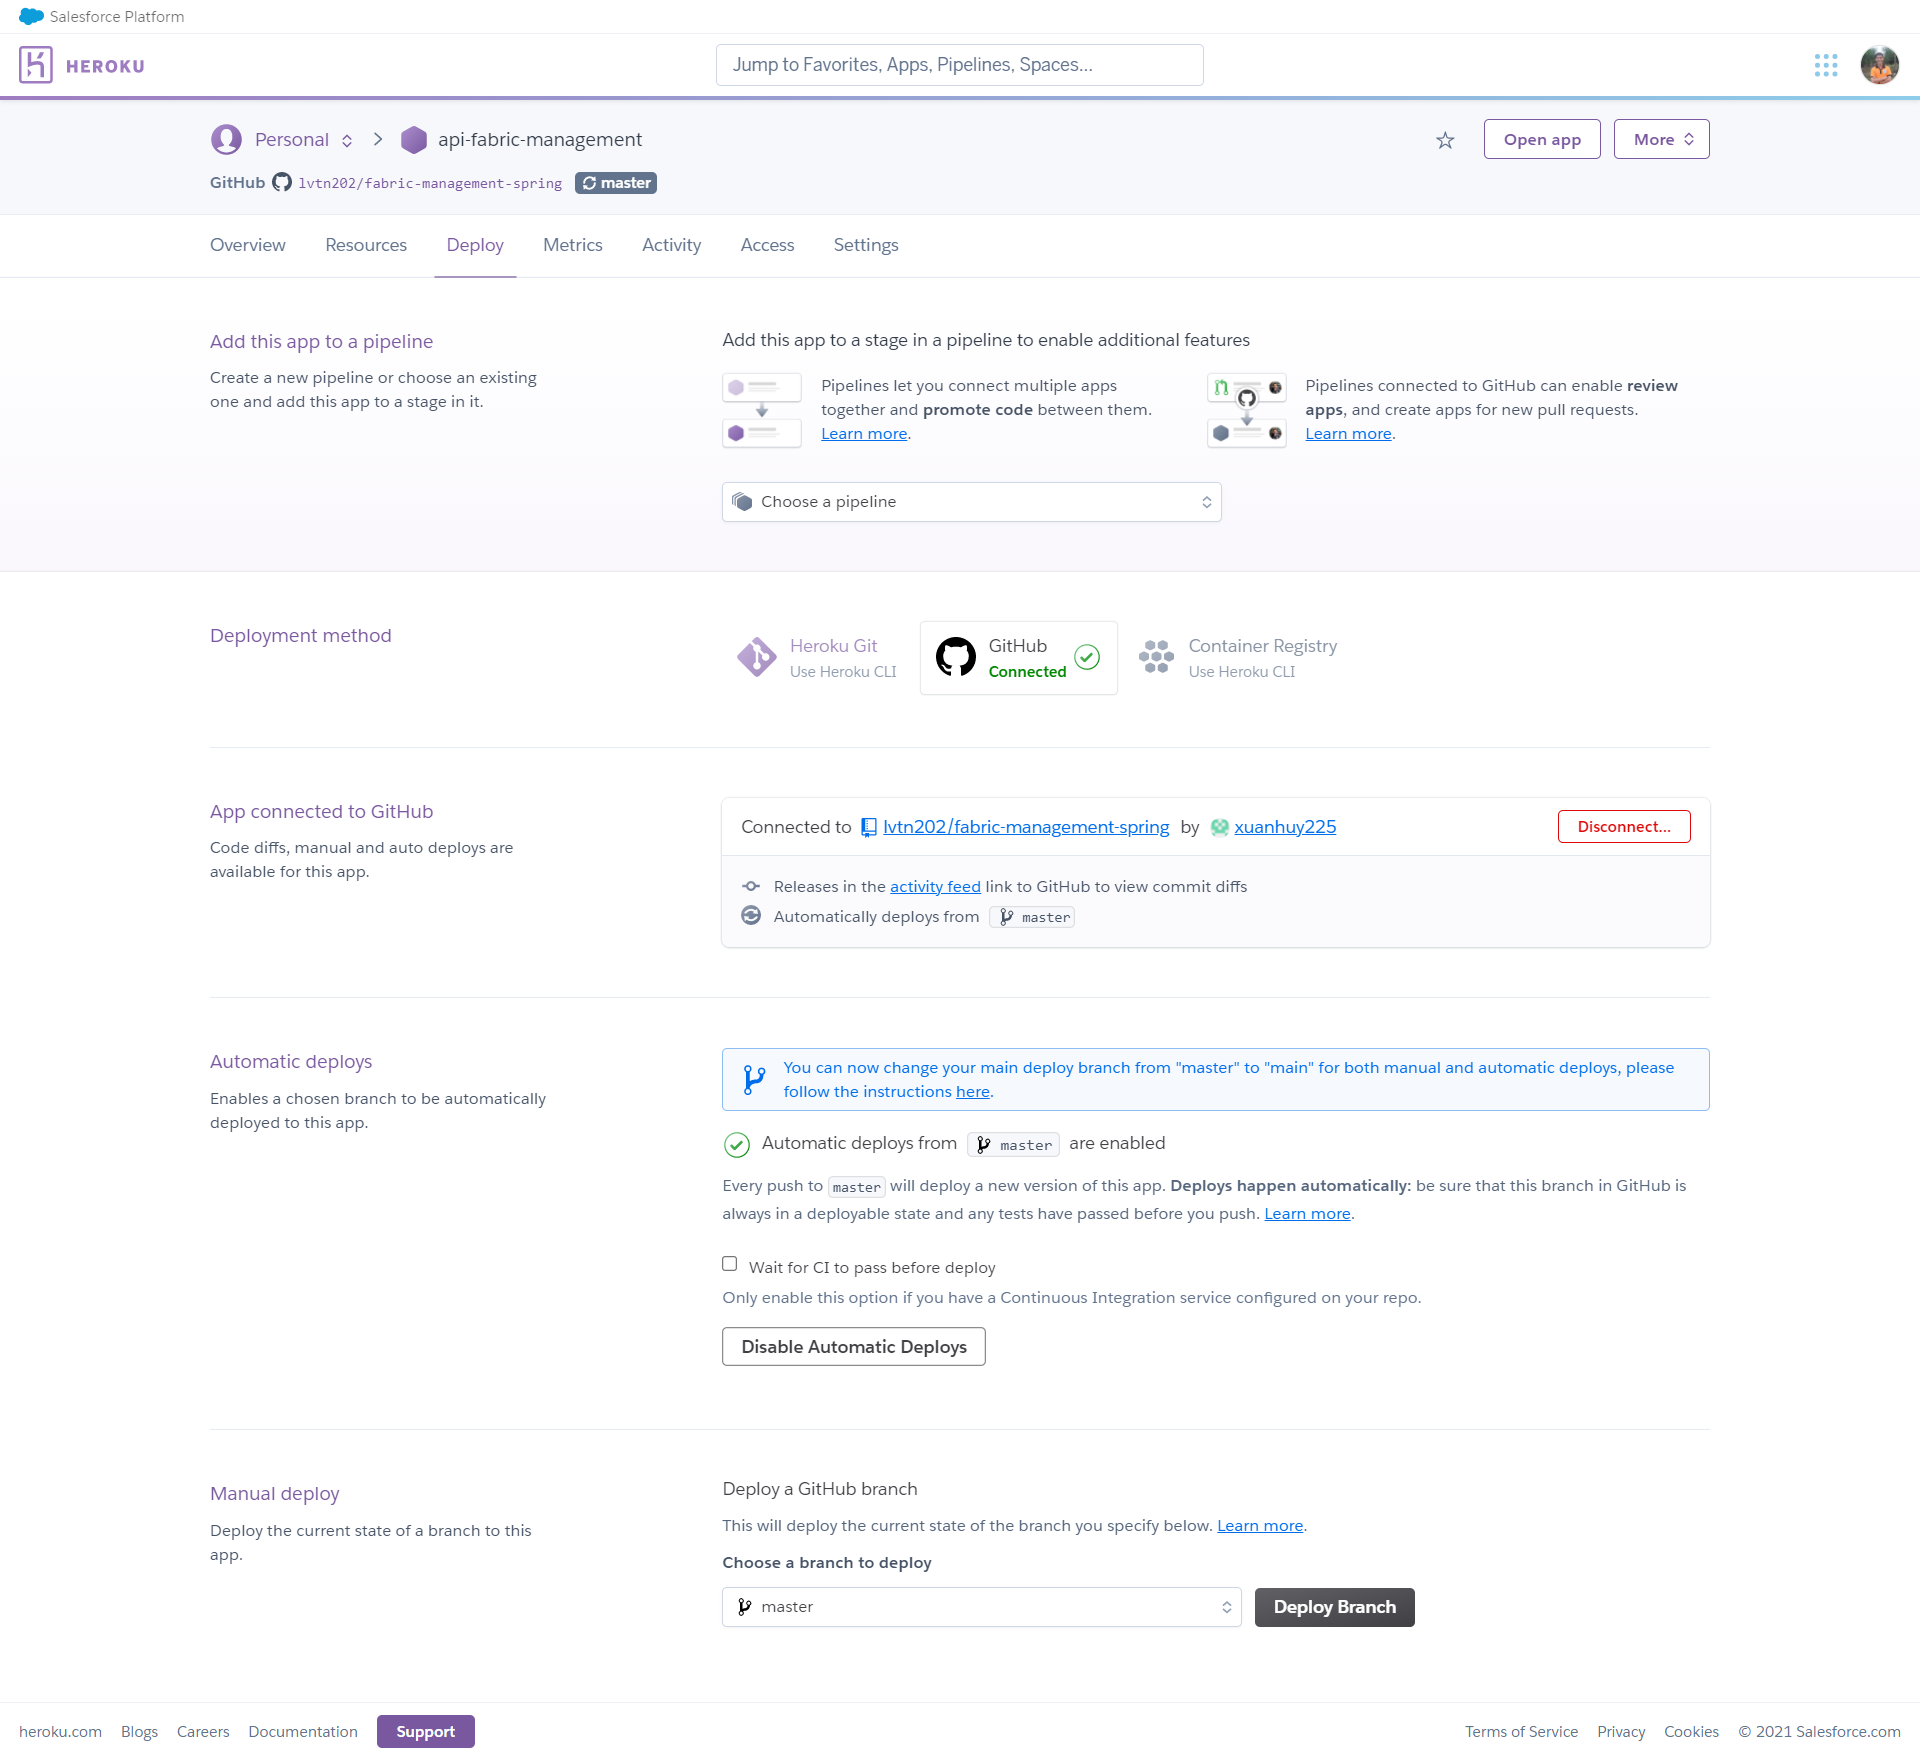
\includegraphics[width=16cm]{Image/Technical/deploy-back-end.png}
        \caption{Deploy Back-end Heroku}
        \label{deploy_back_end}
    \end{center}
\end{figure}